
	This chapter will cover the necessary theoretical background for this
	master thesis and consists of following parts:

	\begin{enumerate}
		\item Graph Theory
		\item Machine Learning on Graphs
		\item Graph Generation
    \end{enumerate}

	\section{Graph Theory}

	This section provides a brief introduction to graph theory, with a focus on
	the relevant aspects for this master thesis. The theory presented is
	primarily taken from the book "Networks: An Introduction" by Mark Newman
	\citeyearpar{Newman2010}. \\

	graph theory is an old field of mathematics and can be traced back to Leonhard Euler and 
	the famous "Königsberg Bridge Problem" \citep{euler1741solutio}, it has 
	experienced a recent revival in machine learning. As it is a relatively 
	novel field in machine learning, it provides for a fruitful ground for 
	testing methods and applications. \\
	

	\noindent Graphs are special data structures as shown in Figure \ref{fig:graph}. The 
	terms graph and network are used inerchangeably for the purpose of this 
	master thesis. Typically, the term graph is used more commonly when referring 
	to mathematical analysis and the term network is more commonly used for data
	science purposes.

	\begin{figure}[h]
		\centering
		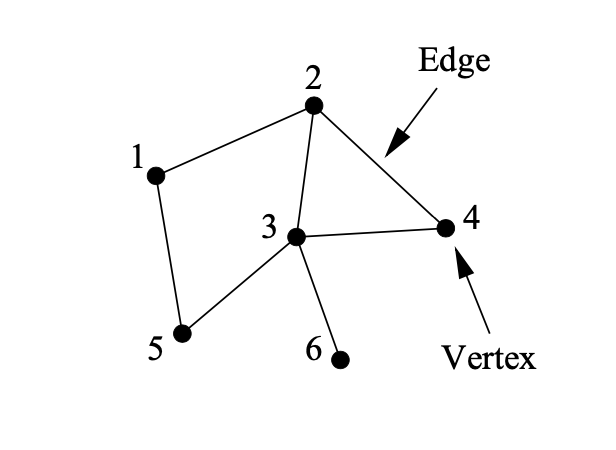
\includegraphics[width=0.5\textwidth]{graph.png}
		\caption{Example of a Graph}
		\cite[p. 111]{Newman2010}
		\label{fig:graph}
	\end{figure}
	
	\noindent The graph shown in Figure \ref{fig:graph} corresponds to an undirected graphs
	in which the connections between the vertexes are mutual. In a directed
	graph for instance, vertex A could be connected to vertex B, however vertex
	B need not be connected to vertex A. For the purpose of this thesis, only
	undirected graphs are considered. Vertexes are commonly reffered to as
	nodes and the terms will be used interchangeably. Edges refer to the
	connections between the vertices. Edges are often also referred to as links
	and the terms will be used interchangeably as well. Graphs may have
	additional elements such as multi-edges or self-edges. These are however
	not relevant for the purpose of this master thesis. \\

	\noindent In terms of mathematical notation, graphs are typically defined
	as follows:

	\begin{equation}
		G(V,E)
	\end{equation}

	\noindent $G$ refers to the graph as an output. $V$ refers to the set of 
	vertices present in the graph and $E$ refers to edges present between the 
	vertices. \\

	\subsection{Adjacency Matrix}

	The adjacency matrix $A$ is defined as a $n \times n$ matrix, where $n$ refers
	to the number of vertices present in the graph. Each vertex is therefore
	recorded by a column and a row in the adjacency matrix. The elements in the
	adjacency matrix are further typically defined as follows:

	\begin{equation}
		A_{ij} = 
			\begin{cases}
				1, & \text{if vertex $i$ and $j$ are connected by an edge} \\
				0, & \text{otherwise}
			\end{cases}
	\end{equation}
	
	\noindent For illustration, the adjacency matrix of the graph shown in Figure
	\ref{fig:graph} is shown as follows:

	\[ A = 
	\begin{pmatrix}
		0 & 1 & 0 & 0 & 1 & 0 \\
		1 & 0 & 1 & 1 & 0 & 0 \\
		0 & 1 & 0 & 1 & 1 & 1 \\
		0 & 1 & 1 & 0 & 0 & 0 \\
		1 & 0 & 1 & 0 & 0 & 0 \\
		0 & 0 & 1 & 0 & 0 & 0  
	\end{pmatrix}
	\] \\
	
	\noindent As one can see, if vertex $i$ and $j$ are connected, this is recorded with
	1 and 0 otherwise. Note, that all the elements on the $diag(A)$ are equal
	to 0. This is because self-edges are excluded. As this is an undirected
	network, the adjacency matrix is symmetric. There are many additonal
	aspects one could mention with regard to the adjacency matrix, they are
	however not relevant for this thesis.

	\subsection{Degree Measures}

	An important measure for graphs are the degrees $k$ of the vertices, the 
	number of edges connected to a vertex. The degrees of vertex $i$ can be 
	formulated as \citep[p.133]{Newman2010}:

	\begin{equation}
		k_i = \sum_{j=1}^{n} A_{ij}
	\end{equation}

	\noindent For an undirected graph, edges have two ends. This is due to the 
	fact that vertices connected by an edge are mutually connected. In terms of 
	the sum of the degrees of all vertices, we can therefore write for a graph 
	with $m$ edges \citep[p.133]{Newman2010}:

	\begin{equation}
		2m = \sum_{i=1}^{n} k_i	
	\end{equation}

	\noindent The sum of all degrees is therefore just the number of edges $m$ 
	multiplied by 2. In terms of statistical measures, the mean degree $c$ of a 
	vertex is defined as follows \citep[p.134]{Newman2010}:

	\begin{equation}
		c = \frac{1}{n}\sum_{i=1}^{n}k_i = \frac{2m}{n}
	\end{equation}

	\noindent In order to define the connectance or density of a graph, we must
	first observe, that the maximum number of edges is given by \citep[p.134]{Newman2010}:

	\begin{equation}
		{n \choose 2} = \frac{1}{2}n(n-1)
	\end{equation}

	\noindent The density $\rho$ can therefore be written as \citep[p.134]{Newman2010}:

	\begin{equation}
		\rho = \frac{m}{{n \choose 2}} = \frac{2m}{n(n-1)} = \frac{c}{n-1}
	\end{equation}

	\noindent Note, that the density $\rho$ lies strictly between 
	$0 \leqslant \rho \leqslant 1$. In addition, for sufficently large graphs,
	one can approximate $\rho = \frac{c}{n}$. 

	\subsection{Eigenvector Centrality}

	The degrees of a vertex shown in the previous section already correspond to
	the simplest form of centrality measures. The issue with this measure
	however is, that the every neighbor of vertex $i$ are valued the same. This
	is a problem, as not all neigbors are of equalt importance due to:

	\begin{enumerate}
		\item Number of neighbors
		\item Importance of neighbor
		\item both
	\end{enumerate}

	\noindent There are many different alternative centrality measures which
	can consider the factors listed above such as eigenvector ecntrality, Katz
	centrality or PageRank
	\citep{katz1953new,page1999pagerank,landau1895relativen,Newman2010}. As we 
	are only dealing with simple undirected graphs, eigenvector centrality will 
	suffice, where the other mentioned methods are adaptations to the 
	eigenvector centrality. \\

	\noindent Eigenvector centrality gives all vertices a score proportional to
	the sum of the scores of its neighbors. This is a procedure in which
	typically the initial centrality $x_i$ of vertex $i$ is guessed to be 1
	$\forall \; i$. This can be used to calculate the centralities of the
	neighbors of $i$ which is denoted as $x_{i}'$. We can thus write
	\citep[p. 169]{Newman2010}:

	\begin{equation}
		x_i' = \sum_{j}A_{ij}x_j
	\end{equation}

	\noindent In matrix form:

	\begin{equation}
		x' = Ax
	\end{equation}

	\noindent This process is repeated $t$ times to provide better estimates
	\citep[p. 170]{Newman2010}:

	\begin{equation}
		x(t) =  A^tx(0)
	\end{equation}

	\noindent Where $x(0)$ is a linear combination of \citep[p. 170]{Newman2010}:

	\begin{equation}
		x(0) =  \sum_{i}c_{i}v_{i}
	\end{equation}

	\noindent $v_i$ correspond to the eigenvectors of the adjacency matrix $A$
	and $c_i$ corresponds to an appropriately chosen constant. Therefore we can
	write \citep[p. 170]{Newman2010}:

	\begin{equation}
		x(t) =  A^t \sum_{i}c_{i}v_{i} = \sum_{i} c_i k_i^t v_i = 
		k_i^t \sum_{i} c_i \left[\frac{k_i}{k_1}\right]^t v_i
	\end{equation}

	\noindent In the above equation, $k_i$ correspond to the eigenvalues of $A$, 
	the adjacency matrix. $k_1$ corresponds to the largest eigenvalue of $A$.
	As $\frac{k_i}{k_1} < 1, \; \forall \; i\neq 1$ , the term is decaying as 
	$t \rightarrow \infty$. The centralities $x$ can therefore be written
	as fulfilling following condition \citep[p. 170]{Newman2010}:

	\begin{equation}
		Ax = k_1 x	
	\end{equation}

	\noindent Lastly, the eigenvector centrality is defined as \citep[p. 170]{Newman2010}:

	\begin{equation}
		x_i = k_{1}^{-1} \sum_{j} A_{ij}x_j 
	\end{equation}

	\subsection{Closeness Centrality}

	Closeness centrality, $C_i$, is defined as the average distance from a vertex to the
	other vertices. This centrality measure is defined as follows \citep[p.
	182]{Newman2010}:

	\begin{equation}
		C_i = \frac{1}{l_i} = \frac{n}{\sum_{j}d_{ij}}
	\end{equation}

	\noindent In this measure, central vertices exhibit high closeness 
	centrality and are therefore closer connected to other vertices compared to 
	vertices with low closeness centrality. $l_i$ refers to the average of the 
	geodesic distances $d_{ij}$ of vertex $i$.

	\subsection{Betweenness Centrality}

	This centrality measures to which extent a vertex lies on paths between
	other vertices. For instance, a bottle neck vertex would exhibit a large
	betweenness centrality as many, if not all nodes must pass through it. More
	formally, betweenness centrality, $x_i$, is defined as \citep[p.
	187]{Newman2010}:

	\begin{equation}
		x_i = \sum_{st} \frac{\eta_{st}^i}{g_{st}}
	\end{equation}

	\noindent In the above equation, $\eta_{st}^i$ refers to the number of 
	geodesic paths from $s$ to $t$ which pass through vertex $i$. Further,
	$g_{st}$ is defined as the number of geodesic paths between vertex $s$ and
	$t$. \\

	\noindent In order to allow for better comparison of betweenness
	centrality, it is often standardized by the number of connected vertex
	pairs $s$ and $t$ denoted as  $\eta^2$. The betweenness centrality
	can therefore be expressed as \citep[p.190]{Newman2010}:

	\begin{equation}
		x_i = \frac{1}{\eta^2}\sum_{st} \frac{\eta_{st}^i}{g_{st}}
	\end{equation}

	\noindent With this measure, the betweenness centrality is within the range
	$0\leqslant1$

	\section{Machine Learning on Graphs}

	\noindent Graph structures are significantly different compared to
	traditional types of data usually used for machine learning tasks or
	regression analyses. Graph structures are special in that the data points
	in a graph have connections with each other. A practical example for this
	are social networks. In a social network, the profiles of "Peter" and
	"Paul" might be connected because Peter and Paul are friends. This aspect
	is unique to graph or network data and provides both additional information
	and additional complexity to graph data not found in other data types. An
	introduction to graph theory will be given in chapter 2.

	\section{Graph Generation}

	It is very difficult to collect graph data, as one cannot capture links
	between observations by traditional data collection means such as surveys. 
	In this regard, banks have a unique advantage (similar to social networks)
	in that they can capture relationships by analyzing their clients cash
	flows. In today's world most people make most if not all of their payments
	electronically and usually pay by card. This provides banks with a large
	amount of information such as spending behavior. Payments are nothing other
	than links in a graph theoretical setting. Unfortunately, access to bank
	client data is rarely granted due to privacy or bank secrecy laws. \\

	\noindent This is a problem for master thesis for which no perfect solution 
	exists. The	search for alternatives lead to graph generation methods. 
	Among the many graph generation algorithms researched, the 
	Multiplicative Attribute Graph (MAG) model appears to provide a feasible 
	solution \citep{kim2012multiplicative}. This model creates probabilistic 
	links between observations using link-affinity matrices. This section will
	provide an introduction to the MAG model. \\
